\documentclass[10pt]{beamer}
\usepackage[utf8]{inputenc}
\usepackage{tikz}
\usepackage{xcolor}
\usepackage{graphicx}
\usepackage{amsmath}
\usepackage{amssymb}
\usepackage{multirow}
\usepackage{caption}
\usepackage{makecell}
\usepackage{multirow}
\usepackage{array}
\usepackage{esint}
\usepackage{adjustbox}
\usepackage{tabularht}
\usepackage{float}
\usepackage{hyperref}
\usepackage{nicefrac}    
\usepackage{microtype}
\usepackage{booktabs}
\usepackage{url}
\usepackage{dsfont}

\usetheme{sleep-states}
\usefonttheme[onlymath]{serif}



\title{\Huge{A Deep Learning approach to detect sleep states}}
\author{Armando Bringas, Alexis Guerrero}
\date{3rd January - 2024}




\begin{document}

\begin{frame}
  \titlepage
\end{frame}

\begin{frame}
  \frametitle{Introduction}
  \begin{block}{Sleep States Detection}
    Our project proposal rooted in the practical application of a Kaggle competition,
aimed at addressing a challenge in pediatric health and neuroscience: the identification of sleep states
in children through wrist-worn accelerometer data \cite{child-mind-institute-detect-sleep-states}.
  \end{block}
  \begin{block}{Project implications}
    The significance of this project lies in its potential to deepen our understanding of sleep and to provide
further insights into its importance. For instance, understanding how environmental factors influence
sleep, mood, and behavior can aid in formulating personalized strategies tailored to the unique needs
of each child.
  \end{block} 
\end{frame}

\begin{frame}
  \frametitle{Literature Review}
  \begin{block}{Models}
    \begin{itemize}
    \item Random Forest
    \item Residual Neural Network (RNN)
    \item Latent Class Analysis (LCA)
    \item Long Short-Term Memory (LSTM)
    \end{itemize}
  \end{block}
  \begin{block}{Data origin}
    \begin{itemize}
    \item Accelerometer data
    \item Actigraphy and sleep diaries
    \item Optical plethysmography
    \item Electrocardiography
    \item Electroencephalography
    \item Multi channel polysomnogram
      \begin{itemize}
      \item Electroculography
      \item Electromyography
      \end{itemize}
    \end{itemize}
  \end{block} 
\end{frame}

\begin{frame}
  \frametitle{Dataset}
  \begin{block}{}
    Dataset consists of approximately 500 multi-day recordings from wrist-mounted accelerometers. The accelerometer data in the dataset was processed using R with the GGIR package \cite{Migueles2019GGIR}. The recordings are labeled with two event types: 'onset', indicating the start of sleep, and 'wakeup', marking its end. The primary objective is to identify these two events within the accelerometer data series, this primarily represents a binary classification task. 
    \begin{figure*}
        \centering
        \includegraphics[width=1\linewidth]{038441c925bb_anglez.png}
        \caption{Accelerometer training data. Plot of \texttt{step} againts \texttt{anglez} showing \texttt{event} state}
        \label{fig:accelerometerdata_series-038441c925bb_anglez}
    \end{figure*}
  \end{block} 
\end{frame}

\begin{frame}
  \frametitle{Model - Random Forest}
  \begin{block}{}
    The Random Forest model is initialized with a predetermined number of 100 estimators (n\textunderscore estimators)
and a minimum leaf sample size (min\textunderscore sample\textunderscore leaf) set to 300. These initial values are chosen for
the purpose of assessing the model’s efficiency and will be subject to subsequent adjustments based
on its performance. Given the substantial volume of data in this scenario, it is anticipated that the
minimum leaf sample size will remain unchanged, whereas the number of estimators will likely need
to be increased to optimize performance. An iteration process is set along the Random Forest model, changing the random\textunderscore state and n\textunderscore estimators values.
\begin{center}
  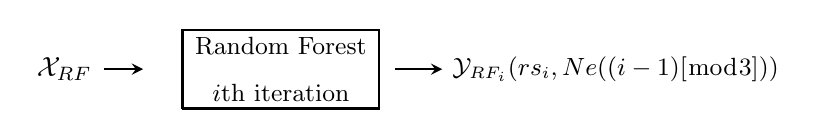
\begin{tikzpicture}
    \node at (0,0) (XRF) {$\mathcal{X}_{RF}$} ;
    \draw[thick, -stealth] (0.5,0) -- (1,0) ;
    \draw[thick] (1.5,-0.5) -- (4,-0.5) -- (4,0.5) -- (1.5,0.5) -- (1.5,-0.5) ;
    \node at (2.75,0.3) {\small{Random Forest}} ;
    \node at (2.75,-0.3) {\small{$i$th iteration}} ;
    \draw[thick, -stealth] (4.2,0) -- (4.8,0) ;
    \node at (7,0) (YRF) {\small{$\mathcal{Y}_{RF_i}(rs_i,Ne((i-1)[\bmod{3}]))$}} ;
  \end{tikzpicture}  
\end{center}
  \end{block} 
\end{frame}

\begin{frame}
  \frametitle{Model - LSTM}
  \begin{block}

        We are proposing a starting neural network architecture with the following blocks where consists of an LSTM layer of 64 units, ideal for processing sequences by capturing dependencies from prior inputs. This is followed by a Dense layer, the size of which matches the number of classification categories in your problem, in this case for our binary classification problem \(n_{\text{classes}} = 2\). The final component is a softmax activation function, applied to convert the output into a probability distribution across the predicted classes. 
        \begin{figure}[h]
          \centering
          \[
          \xrightarrow{\text{input}} \boxed{\text{LSTM} (64)} \rightarrow \boxed{\text{Dense} (n_{\text{classes}})} \xrightarrow{\text{softmax}}
          \]
          \caption{Neural Network for accelerometer data classification}
          \label{fig:neuralnetwork}
        \end{figure}
  \end{block} 
\end{frame}

\begin{frame}
  \frametitle{Evaluation Metrics}
  \begin{block}{Average Precision}
    \begin{gather*}
  \text{Inputs} \ \mathcal{X} = (x_1, \ldots, x_N)^\intercal \\
  \text{Outputs} \ \mathcal{Y} = (y_1, \ldots, y_N)^\intercal \\
  \text{Labels} \ \mathcal{W} = (w_1, \ldots, w_N)^\intercal 
    \end{gather*}

    \begin{equation*}
      AP = \frac{1}{N} \sum_{i=1}^{N}{\mathcal{C}(w_i,y_i)}
    \end{equation*}

    \[
    \mathcal{C}(w_i,y_i) =
    \begin{cases}
      1 \text{ if } w_i = y_i \forall i \in \mathds{N}, 1 \leq i \leq N\\
      0 \text{ if } w_i \neq y_i \forall i \in \mathds{N}, 1 \leq i \leq N
    \end{cases}
    \]
    \begin{equation*}
      APF(\mathcal{W}, \mathcal{Y}) = \frac{1}{N} (\omega_1, \ldots, \omega_N) (1, \ldots, 1)^\intercal
    \end{equation*}
  \end{block} 
\end{frame}

\begin{frame}
  \frametitle{Evaluation Metrics}
  \begin{block}{Specificity and Recall}
    \[
    \text{Score}(x) = 
    \begin{cases} 
      \text{TP} & \text{if }x \text{ matched and } x > \text{thresh.} \\
      \text{FP} & \text{if }x \text{ unmatched pred.} \\
      \text{FN} & \text{if }x \text{ unmatched truth} \\
      \text{TN} & \text{otherwise}
    \end{cases}
    \]
    \begin{equation*}
      \text{Specificity} = SPC = \frac{TP}{TP+FN} \hspace{5mm} \text{Recall} = SN = \frac{TN}{TN+FP}
    \end{equation*}
  \end{block}
  \begin{block}{Final evaluation}
    \begin{equation*}
      \text{Model evaluation } = \alpha APF + \beta SPC + \gamma SN 
    \end{equation*}
  \end{block}
\end{frame}

\begin{frame}
    \frametitle{Results}
    \begin{block}{}
        Due to computing performance implications we perform training and evaluation in a reduced dataset consisting in 35 recording out of the 500 recording provided as well by the Kaggle competition.
    \end{block}
    
    \begin{block}{}
        \begin{table}[h]
            \centering
            \caption{Random Forest Confusion Matrix}
            \label{tab:random_forest_confusion_matrix}
            \begin{tabular}{lcc}
                \hline
                \textbf{Actual / Predicted} & \textbf{Predicted Negative} & \textbf{Predicted Positive} \\
                \hline
                \textbf{Actual Negative} & 786677 (31.38\%) & 56959 (2.27\%) \\
                \textbf{Actual Positive} & 70514 (2.81\%) & 1592674 (63.53\%) \\
                \hline
            \end{tabular}
        \end{table}

        \begin{table}[h]
            \centering
            \caption{LSTM Confusion Matrix}
            \label{tab:lstm_confusion_matrix}
            \begin{tabular}{lcc}
                \hline
                \textbf{Actual / Predicted} & \textbf{Predicted Negative} & \textbf{Predicted Positive} \\
                \hline
                \textbf{Actual Negative} & 813470 (32.45\%) & 30166 (1.20\%) \\
                \textbf{Actual Positive} & 178414 (7.12\%) & 1484774 (59.23\%) \\
                \hline
            \end{tabular}
        \end{table}
    \end{block} 
\end{frame}

\begin{frame}
    \begin{block}{}
        Random Forest slightly outperformed LSTM in the Confusion Matrix for Accuracy, Recall, and Specificity metrics. However, concerning model training computational performance, Random Forest took approximately 1 hour to train a single iteration, compared to LSTM, which took approximately 10 minutes to train all defined epochs.
    \end{block}
    \frametitle{Results}
    \begin{block}{}
        \begin{table}[h]
            \centering
            \caption{Model Comparison}
            \label{tab:model_comparison}
            \begin{tabular}{lccccc}
                \hline
                \textbf{Metric} & \textbf{Random Forest} & & \textbf{LSTM} & \\
                \cline{2-5}
                Accuracy & 0.95 & & 0.92 & \\
                Recall & 0.96 & & 0.90 & \\
                Specificity & 0.96 & & 0.97 & \\
                Average Precision & 0.99 & & 0.99 & \\
                Partial Evaluation & 0.96 & & 0.95 & \\
                \hline
            \end{tabular}
        \end{table}
    \end{block} 
\end{frame}

\begin{frame}
  \frametitle{Conclusion}
  \begin{block}{}
    In conclusion, our findings underscore the importance of considering both performance metrics and computational efficiency when selecting a model for sleep state detection. Moreover, our exploration underscores the intricate nature of sleep state detection, compounded by the diverse origins of data stemming from various devices, making data sources a relevant point to take into consideration when selecting a model. Additionally, the need for context-specific solutions and the exploration of advanced architectures indicate exciting avenues for future research in this field, enhancing accessibility to personalized care tailored to the unique characteristics of each patient in the study of sleep.
  \end{block} 
\end{frame}


\begin{frame}
  \frametitle{Bibliography}
  \begin{block}{}
    {
        \small
        %%%%%%%%%%%%%
        \bibliographystyle{plainnat} % or another suitable style
        \bibliography{bibliography} % replace with your BibTeX file name
    }
  \end{block} 
\end{frame}

\end{document}
